\chapter{Analisi del problema \& Progettazione}\label{ch:project}
  Una volta chiariti i requisiti del sistema, il passo successivo riguarda la progettazione dello stesso.
  In particolare, occorre delineare più nel dettaglio l'architettura di massima del sistema, per poi spostare l'attenzione su ciascuna entità interagente.

  % \section{Architettura del sistema}
  Come preventivato già in fase di analisi dei requisiti, il sistema vede la presenza di due principali entità:

  \begin{itemize}
    \item una pagina web che costituisce il client del sistema.
    \item un server di backend, che esegue su piattaforma JVM interfacciandosi con un esecutore di codice Protelis.
  \end{itemize}

  \begin{figure}[htbp]
    \centering
    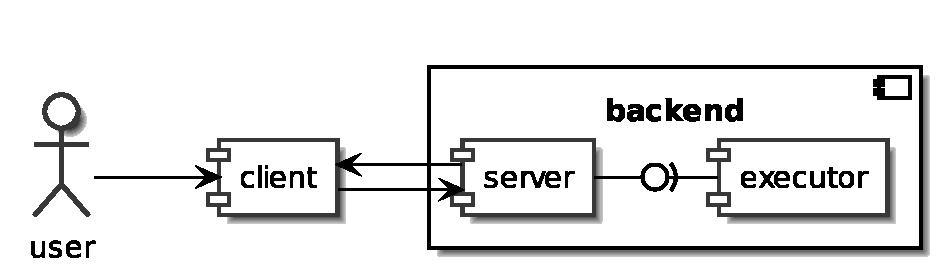
\includegraphics[width=.8\textwidth]{res/uml/architecture-design.eps}%
    \caption{Il diagramma UML riporta l'architettura di massima dei componenti del sistema}%
    \label{fig:architecture-design}
  \end{figure}

  Nelle \nameCrefs{sec:arch:client} successive di questo \nameCref{ch:project}, si intende analizzare più nel dettaglio questa struttura (della quale si ha una rappresentazione grafica in~\Cref{fig:architecture-design}),
  focalizzandosi sui dettagli di ciascun componente.

  \section{Design dell'applicazione}\label{sec:client-design}
    % TODO: inserire breve introduzione sulle GUI

    \subsection{Mockup dell'interfaccia}\label{subsec:mockup}
      Una volta chiariti i requisiti e le possibili fonti di ispirazione per la struttura della UI da realizzare, sono stati disegnati dei mockup che potessero rappresentare una linea guida
      per l'implementazione concreta dell'interfaccia.

      Come detto anche nella~\Cref{subsec:online-ide}, la struttura grafica dell'applicazione dovrebbe ispirarsi a quella di altri ambienti di sviluppo online,
      come ad esempio Overleaf (\Cref{fig:overleaf}).

      \begin{figure}[htbp]
        \centering
        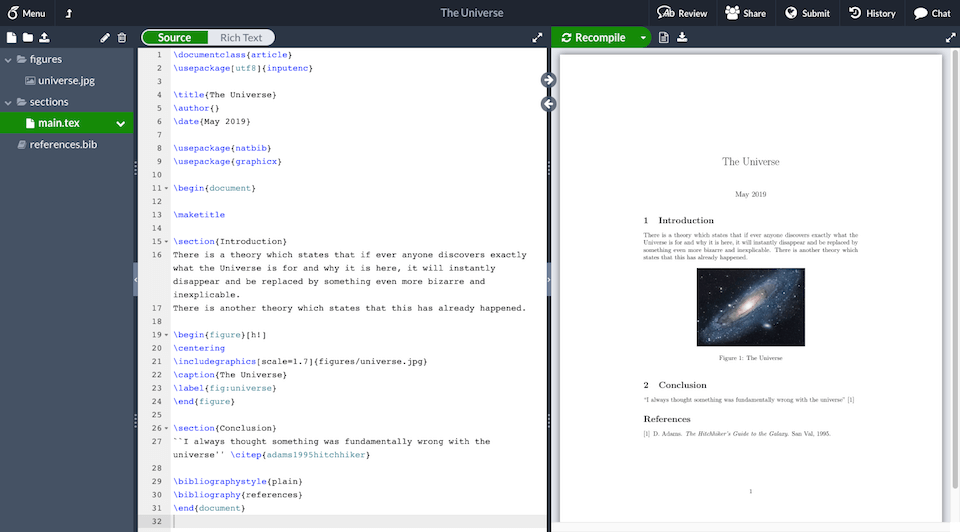
\includegraphics[width=.85\textwidth]{res/fig/overleaf.png}%
        \caption{Screenshot prelevato dalla pagina principale della web app Overleaf}%
        \label{fig:overleaf}
      \end{figure}

      Tali applicazioni hanno generalmente una struttura bipartita:
      nella parte sinistra è solitamente presente un editor che ricorda quello disponibile in diverse IDE desktop, mentre nella parte destra viene generalmente inserita una visualizzazione dell'output.
      Ad esempio, in Overleaf è possibile, alternativamente, visualizzare il log degli errori o il documento compilato.

      \begin{figure}[htbp]
        \centering
        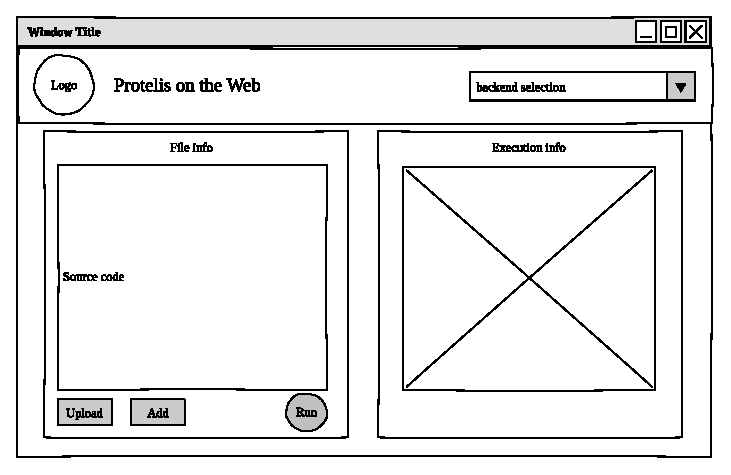
\includegraphics[width=.85\textwidth]{res/mockup/gui-actual.eps}%
        \caption{Mockup dell'interfaccia che dovrà presentare la pagina web}%
        \label{fig:mockup}
      \end{figure}

      Nel mockup finale, riportato in~\Cref{fig:mockup}, si è preso molto ispirazione da questo tipo di struttura.
      L'interfaccia dovrebbe infatti essere costituita dalle parti seguenti:

      \begin{itemize}
        \item
          Una \emph{barra superiore}, nella quale è riportato il nome e il logo del progetto, insieme a un selettore per il backend.
          Nei primi mockup, tale selettore era posizionato nella sezione principale della pagina, ma successivamente si è preferito spostarlo per sfruttare al meglio lo spazio a disposizione.
        \item
          Un \emph{blocco di sinistra}, che costituisce la parte con cui l'utente può interagire per lavorare sul codice.
          Il componente principale è appunto l'editor, un campo di testo avanzato che permette di visualizzare il codice Protelis di esempio e modificarlo.
          Sotto di esso sono presenti i bottoni di controllo per interagire con l'esecuzione.
        \item
          Un \emph{blocco di destra}, che ospita un canvas in cui l'esecuzione viene rappresentata.
          Al suo interno verranno visualizzati i nodi su cui il codice sta eseguendo.
          % In questa sezione, i componenti principali sono:
          % \begin{description}
          %   \item[Editor]
          %     Un campo di testo in cui visualizzare codice Protelis di esempio e modificarlo.
          %   \item[Play]
          %     Un bottone che permette di lanciare l'esecuzione del codice.
          %   % \item[Add]
          %   % TODO
          % \end{description}
      \end{itemize}

    \subsection{Design di riferimento}\label{subsec:material}
      Come è stato già sottolineato, l'applicazione vede come utilizzo principale quello dell'utente inesperto del linguaggio.
      L'interfaccia non deve essere solo semplice, ma anche moderna, gradevole e intuitiva.
      Era dunque necessario scegliere uno stile grafico familiare, moderno e facilmente adattabile a quella che sarebbe essere la nuova interfaccia che si stava progettando.

      Prendendo come esempio l'interfaccia di Overleaf (\Cref{fig:overleaf}), è possibile notare come il design di base abbia uno stile di tipo \emph{flat};
      si è deciso dunque di valutare tra i principali design possibili quali fosse più adeguato per la UX che si aveva intenzione di progettare.

      La scelta è infine ricaduta sul Material Design sviluppato da Google:
      dal suo annuncio nel giugno del 2014 al Google I/O 2014 Keynote esso è stato almeno parzialmente adottato in molte applicazioni web, mobile e desktop
      e ben si si presta all'implementazione di un'interfaccia semplice e minimale. % TODO eventualmente cita evoluzioni successive

      Per offrire un'esperienza coerente, si è deciso di utilizzare le icone e le direttive in merito a dimensioni e variazioni nella palette di colori fornite da Google\footnote{\url{https://material.io}}.
      Il colore base utilizzato per generare la palette è stato ricavato dall'icona ufficiale di Protelis. % TODO: cite logo

  \section{Architettura del client}\label{sec:arch:client}

    L'applicazione web che svolge il ruolo di client è a tutti gli effetti un'applicazione indipendente dotata di interfaccia grafica.
    % Sono stati valutati i numerosi pattern di modellazione documentati in letteratura e, alla fine,
    Sono numerosi i pattern di modellazione documentati in letteratura.
    % Molti di questi (genericamente definiti ``MV*'', ossia \emph{\emph{M}odel, \emph{V}iew} e qualsiasi cosa, generalmente \emph{Controller} o \emph{ViewModel}) tendono a distinguere entità che modellano il dominio
    % Tra tutti quelli considerati, si è scelto di adottare il \emph{pattern Flux} nella variazione chiamata \emph{pattern Redux}.
    La caratteristica maggiormente ricercata durante la progettazione è la reattività:
    il sistema dovrebbe aggiornarsi rapidamente sia quando l'utente lo richiede, interagendo via browser, sia quando il server manda un aggiornamento.

    % È stato dunque ritenuto necessario scegliere un approccio che ponesse al centro lo \emph{stato} del sistema, per poi scegliere, nella prossima fase, le tecnologie più adatte a reagire rapidamente alle sue variazioni.

    % Nelle \nameCrefs{subsec:state-manage} che seguono verranno prese in considerazione le scelte fatte decidendo il piano di lavoro.

    \subsection{Framework di sviluppo}\label{subsec:react}

      Sono disponibili numerosi framework per lo sviluppo di applicazioni web \emph{single-page}, ciascuna dei quali ottimizzata per determinati pattern di progettazione.
      Essendo un requisito la realizzazione di una SPA, la scelta di quale framework impiegare è fondamentale già in fase di progetto, in quando può notevolmente condizionare il piano di lavoro.

      Per l'implementazione di questo prototipo, è stato scelto il framework React, sviluppato da Facebook e compatibile, ufficialmente o meno, con numerosi linguaggi.
      Tecnicamente React, senza prendere in considerazione gli strumenti sviluppati intorno ad esso, sarebbe una libreria per la costruzione di pagine web reattive e \emph{data-driven};
      esso potrebbe essere considerato, riduttivamente, il \emph{view layer} dei pattern architetturali \emph{MV*} (\emph{Model View Anything}).
      React non è però vincolato al pattern MVC come AngularJS o a MVVM come Angular dalla versione 2 in poi.

      % In AngularJS, ogni vista è associata ad un controller, che si occupa della gestione dei dati e della loro visualizzazione.
      % La view è definita da un template, formata da elementi HTML, ed è compito dello sviluppatore associare la logica di controllo alla rappresentazione.

      La divisione principale che determina la struttura è quella tra \emph{componenti}.
      In React, un componente è un'astrazione che incapsula i dati, la loro manipolazione e la logica di rappresentazione e va a definire il più piccolo elemento costitutivo dell'applicazione.
      Esso rimuove la necessità del \emph{data-binding} tra modello e vista, tipico dei pattern MV*, e mantiene la logica applicativa all'interno di ciò a cui fa riferimento.

      Un componente definisce insomma cosa deve essere renderizzato;
      il sistema, autonomamente, determina in modo reattivo quando una delle dipendenze è cambiata e il componente può essere singolarmente ridisegnato.

      In questo modo, è possibile costruire applicazioni componendo tra loro questi elementi in una struttura simile a un albero, delegando la logica di gestione al motore di React, che se ne occuperà in modo efficiente.

      La progettazione dell'architettura deve dunque spostarsi sulla gestione dello stato.

      % React, come buona parte dei framework per lo sviluppo di applicazioni web, si basa sul concetto di \emph{componente}.
      %
      % Il successo di React deriva dalla visione innovativa della struttura di un'applicazione web.
      % React non presenta una separazione netta tra gli elementi di vista, presentazione e logica applicativa;

      % non esiste un controller, né data-binding

      % Anziché separare in modo deciso gli elementi di vista dal resto della logica applicativa (come invece accade tramite template e linguaggi di markup in Angular, ad esempio),

      % React incapsula
      % L'approccio tradizionale, adottato ad esempio da Angular, utilizza dei template realizzati tramite linguaggi di markup, dove la vista è realizzata tramite , sul quale vengono fatti

      % React nasce fondamentalmente come risposta al problema del \emph{change detection} che affligge.

      % start TODO
      % È stato dunque ritenuto necessario scegliere un approccio che ponesse al centro lo \emph{stato} del sistema, per poi scegliere, nella prossima fase, le tecnologie più adatte a reagire rapidamente alle sue variazioni.
      % end TODO

    \subsection{Pattern di gestione dello stato}\label{subsec:state-manage}
  Durante la fase di progettazione di un sistema software, è fondamentale definire la struttura con la quale le singole componenti saranno organizzate.

  Nel contesto applicativo di software orientati all'interazione con l'utente tramite interfaccia grafica, come ad esempio un'applicazione web,
  è spesso consigliato definire chiaramente la gestione dello stato e del flusso informativo, quando questi non sono imposti da eventuali framework utilizzati.

  Per esempio, come accennato nella~\Cref{subsec:react}, React prevede che la struttura dei componenti sia definita da un albero:
  lo stato di questi può fluire solo verso il basso, dunque si consiglia di mantenerlo il più alto possibile nella gerarchia;
  si parla infatti di ``\emph{state lift-up}''.
  Questo tipo di soluzione può risultare limitante in caso di un numero elevato di componenti, dunque sono stati elaborati pattern specifici per la gestione dello stato.

  \subsubsection{Flux architecture}
    Come alternativa al più classico \emph{Model-View-Controller} (MVC)~\cite{Reenskaug2003TheM},
    Facebook propone per le applicazioni React un nuovo pattern architetturale denominato Flux~\cite{10.1145/2742580.2742818}.
    Esso sottolinea la natura unidirezionale del flusso di dati in un'applicazione React (di qui il nome)
    e può essere di fatto considerato una variante del \emph{pattern Observer}~\cite{10.5555/186897} applicato all'architettura del sistema.

    \begin{figure}[htbp]
      \centering
      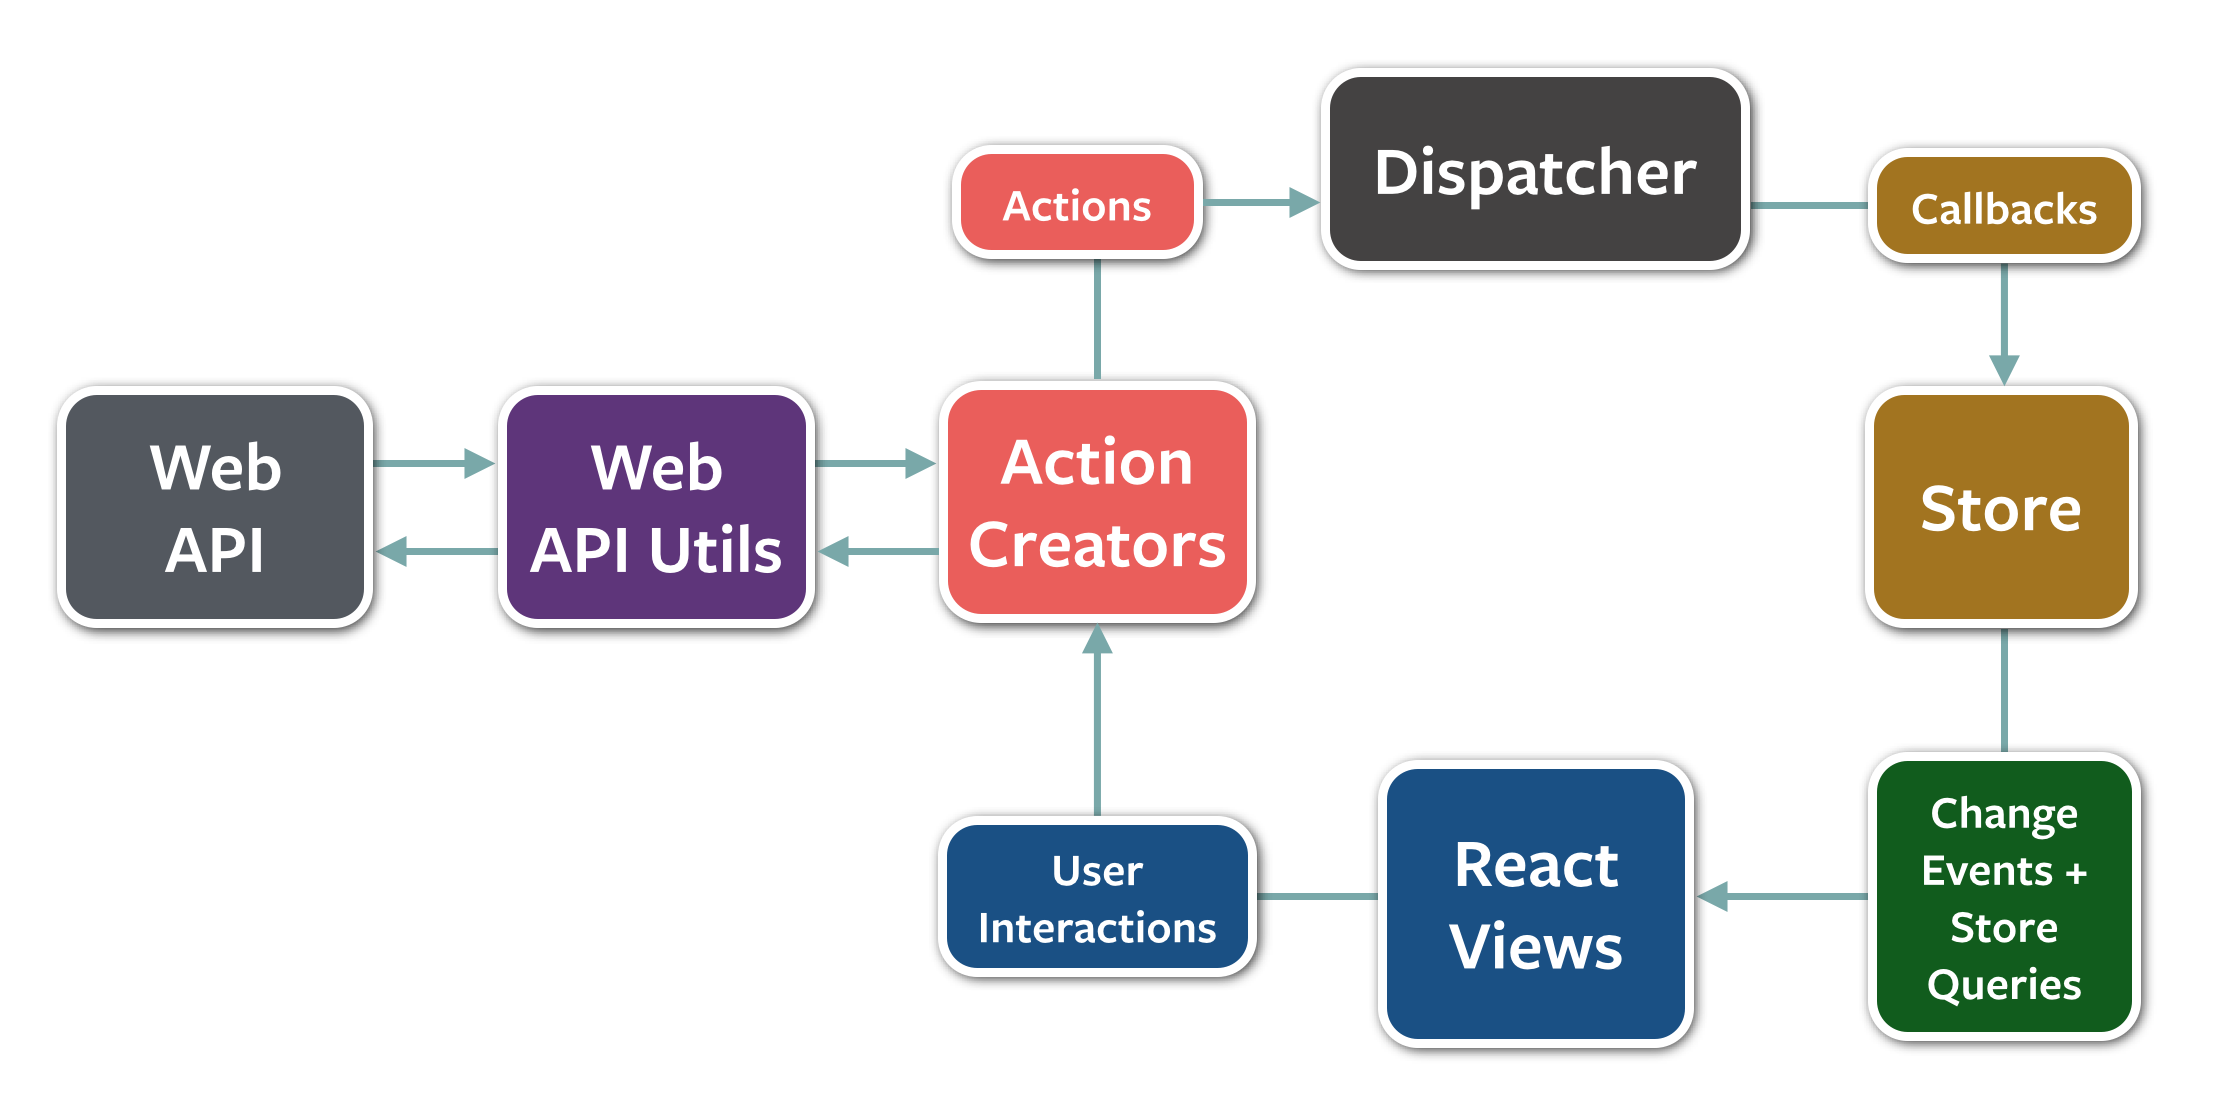
\includegraphics[width=.9\textwidth]{res/fig/flux-diagram-white-background.png}
      \caption[
        Rappresentazione del flusso unidirezionale dei dati in un'applicazione React con Flux.
      ]{
        Rappresentazione del flusso unidirezionale dei dati in un'applicazione React con Flux.
        Figura ripresa dalla documentazione ufficiale.
      }%
      \label{fig:flux}
    \end{figure}

    Come è possibile vedere in~\Cref{fig:flux}, la struttura è composta da quattro entità principali:
    \begin{description}
      \item[Store]
        Rappresenta il ``contenitore'' che incapsula lo \emph{stato} (del dominio applicativo e/o dell'interfaccia grafica).
        Ciascuno store agisce come \emph{single source of truth} (SSOT)
        e non permette di modificare direttamente i valori dello stato, ma solo tramite \emph{azioni} passate con un \emph{dispatcher}.
      \item[Dispatcher]
        Singolo oggetto che invia in broadcast come eventi le azioni agli store;
        gli store devono essere registrati per gli eventi che sono in grado di gestire all'avvio dell'applicazione.
      \item[View]
        Rappresenta la componente di interazione con l'utente;
        essa osserva gli store per aggiornarsi al variare dello stato e genera azioni sulla base delle richieste dell'utente.
        Sono possibili due tipi di view:
        \begin{description}
          \item[Presentation view] Non si collega né al dispatcher, né agli store, bensì comunica tramite \emph{proprietà} definite alla costruzione.
          \item[Container view] Si collega al dispatcher e/o agli store, reagendo agli eventi e/o generandoli.
        \end{description}
      \item[Action]
        Oggetto semplice e immutabile che contiene tutte le informazioni necessarie per modellare un'interazione con lo stato.
        Possono essere generate dalla view o da API web esterne, ma sempre attraverso un \emph{action creator}.
    \end{description}

    Il flusso informativo avviene dunque in una singola direzione e tramite \emph{callback}.
    Questo garantisce le seguenti proprietà:

    \begin{description}
      \item[Asincronismo]
        Il motore che interpreta JavaScript gestisce ciascuna callback eseguendola al ciclo successivo, non bloccando l'esecuzione attuale.
      \item[Consistenza di rappresentazione]
        Essendo ciascuno store centralizzato per l'intera applicazione, lo stato rappresentato dovrebbe essere univoco indipendentemente dalla pagina attuale.
      \item[Disaccoppiamento]
        Essendo lo store esterno ai componenti grafici, essi risultano maggiormente disaccoppiati rispetto al dominio e più riusabili.
      \item[Determinismo]
        Essendo lo stato aggiornabile solo tramite azioni, non si hanno effetti secondari e l'applicazione risulta più facile da rappresentare come una sequenza finita di stati, agevolando anche la fase di testing.
    \end{description}

  \subsubsection{Redux pattern}

    Il pattern Redux è una delle più popolari varianti del pattern Flux.

    Redux\footnote{\url{http://redux.js.org}} è il nome della libreria JavaScript per la gestione dello stato che per prima ne ha definito un'implementazione.
    Creata da Dan Abramov e Andrew Clark nel 2015 come implementazione alternativa a quella ufficiale del pattern Flux,
    essa combina idee provenienti dal pattern \emph{Command}~\cite{10.5555/186897} e dall'\emph{architettura Elm} teorizzata con l'omonimo linguaggio~\cite{czaplicki2012elm}:
    lo stato dell'applicazione è descritto da un singolo POJO (\emph{Plain Old JavaScript Object}) all'interno dello store e gli aggiornamenti avvengono tramite \emph{reducer}, funzioni pure di un'azione e dello stato corrente che generano un nuovo stato.

    \begin{figure}[htbp]
      \centering
      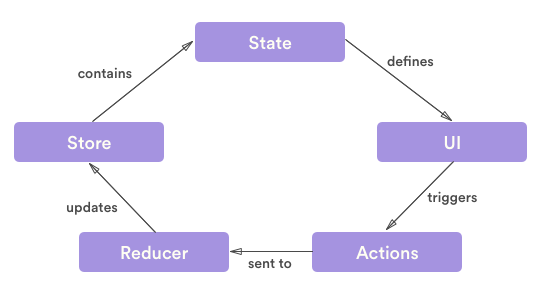
\includegraphics[width=.9\textwidth]{res/fig/redux-diagram.png}
      \caption[
        Rappresentazione del flusso unidirezionale dei dati in Redux.
      ]{
        Rappresentazione del flusso unidirezionale dei dati in Redux.

        Figura ripresa dalla documentazione ufficiale.
      }%
      \label{fig:redux}
    \end{figure}

    Secondo la documentazione ufficiale, la completa centralizzazione dello stato permette al sistema di essere completamente predicibile, permettendo il ``\emph{time-travel debug}'' tramite strumentazione integrata nel browser.
    Inoltre, il non essere strettamente legato a un framework di rappresentazione e la possibilità di caricare middleware lo rendono estremamente flessibile.

      Nel caso di questo progetto, tale soluzione è stata ritenuta ottimale per il tipo di architettura che si intende realizzare.

      Prendendo dunque in considerazione il mockup delineato alla~\Cref{subsec:mockup}, lo store sarebbe costituito dalle seguenti parti (dette \emph{slice}):

      \begin{description}
        \item[Editor]
          In \texttt{editorSlice} saranno inserite tutte le informazioni relative allo stato dei file.
          In particolare, è possibile definire al suo interno una struttura ad albero riguardante i file e lo stato di apertura degli stessi.
        \item[Esecuzione]
          In \texttt{execSlice} saranno invece inseriti i dati relativi all'esecuzione, come:
          \begin{itemize}
            \item lo stato della connessione,
            \item lo stato della simulazione,
            \item l'ID della simulazione,
            \item i dati dei nodi da rappresentare.
          \end{itemize}
      \end{description}

      \improvement[inline]{
        Mi piacerebbe aggiungere maggiori dettagli ``formali'', ad esempio graficamente con UML, ma non saprei come.

        Da quanto leggo online, non è esattamente il tipo di grafico adatto a questo tipo di pattern architetturale.
      }

  \section{Architettura del server}\label{sec:arch:server}

    Il server costituisce l'entità del sistema che si occupa dell'esecuzione del codice Protelis; è un esecutore remoto.

    Innanzitutto, è stato necessario chiarire se l'architettura dovesse essere monolitica o separata in microservizi.
    In tempi recenti, l'approccio a microservizi viene preferito a causa di diversi vantaggi:

    \begin{itemize}
      \item
        un sistema composto da microservizi indipendenti è più semplice da scalare,
        in quanto è possibile replicare ciascun servizio in modo indipendente dagli altri, a seconda delle esigenze.
      \item
        l'approccio a microservizi risulta generalmente più semplice da manutenere,
        in quanto disaccoppia i servizi tra loro, rendendo chiare le dipendenze condivise e permettendo lo sviluppo indipendente delle componenti.
      \item
        offrono un'integrazione migliore con orchestratori cloud e permettono di impiegare tecnologie di \emph{continuous deployment} (CD) in modo più efficiente.
    \end{itemize}

    Tali vantaggi sono però maggiormente evidenti quando le funzionalità che devono essere offerte sono \emph{tante}.
    Nel caso di questo progetto, di contro, il sistema deve essere in grado di gestire in modo efficiente un solo tipo di servizio, ossia l'esecuzione di codice su una rete simulata.

    In questo caso, dunque, è stato ritenuto più adeguato scegliere un'architettura monolitica, favorendo la semplicità di progettazione
    e delegando la gestione dello scaling al livello di piattaforma di deploy.

    \subsection{Pattern reactor}\label{subsec:reactor}

      Il giusto livello di reattività ed efficienza è stato trovato nell'approccio \emph{event-driven} con \emph{event-loop}.
      Tramite questo modello di concorrenza, denominato \emph{pattern Reactor}~\cite{Schmidt1995ReactorAO}, il server gestisce le richieste dei client attraverso una coda:
      uno o più cicli si occupano di gestire gli eventi nella coda in modo sincrono.
      In particolare, si è deciso di adottare il modello \emph{multi-reactor} fornito da Vert.x.

      \emph{Vert.x} è un framework applicativo event-driven che esegue su JVM (nonostante offra un supporto poliglotta a diversi linguaggi).
      Del modello architetturale messo a disposizione dal framework, è stato considerato interessante il concetto di \emph{Verticle}:
      esso è un'astrazione che incapsula un event-loop insieme al suo stato e interagisce tramite gli eventi provenienti da un event-bus.
      La documentazione\footnote{\url{https://vertx.io/docs/vertx-core/kotlin/\#_verticles}} % TODO: move to biblio
      specifica che l'approccio non può essere considerato pienamente \emph{ad attori}, bensì solo \emph{actor-like}.

      Per questo progetto, il modello è stato considerato adatto, in quanto in grado di garantire il giusto livello di astrazione e i criteri di reattività richiesti.

    \subsection{Verticle individuati}
      Il sistema progettato è composto da due componenti principali.

      \begin{itemize}
        \item
          Il primo, chiamato \texttt{BridgeVerticle}, è dedicato alla gestione delle API per la comunicazione da e verso l'esterno.
          % Esso si avvale dell'EventBus di Vert.x per comunicare con l'esterno
          In particolare, esso implementa il pattern \emph{bridge} relativamente alle connessioni verso l'esterno, trasformando le chiamate HTTP eseguite dai client in eventi espliciti dell'EventBus.
          % In questo modo, all'interno dell'applicazione, tutte le istanze dei verticle interessati possono essere
          Gestendo le comunicazioni con l'esterno, esso astrae l'intero processo di gestione del protocollo di comunicazione dalle altre componenti dell'applicazione.
        \item
          Il secondo è invece chiamato \texttt{AlchemistVerticle} e costituisce l'entità che si interfaccia con un motore di esecuzione esterno,
          come detto nell'architettura generale delineata all'inizio di questa fase di progettazione (\Cref{fig:architecture-design}).
          In particolare, per eseguire il codice si è scelto di utilizzare il simulatore Alchemist, che verrà analizzato più nel dettaglio nella~\Cref{subsec:alchemist}.
      \end{itemize}

      Oltre a questi, è stato anche progettato l'uso di un verticle principale \texttt{MainVerticle}, che viene lanciato dall'avviatore di Vert.x e che coordina l'avvio dei due verticle descritti sopra.

    \subsection{Simulatore scelto: Alchemist}\label{subsec:alchemist}
  Alchemist~\cite{alchemist-jos2013} è un meta-simulatore estendibile completamente \emph{open-source} che esegue su \engEmph{Java~Virtual~Machine}, nato all'interno dell'Università di Bologna.

  \subsubsection{Simulazione}\label{subsec:introAlchemist}
    In generale, una \emph{simulazione}~\cite{des3} è una riproduzione del modo di operare di un sistema o un processo del mondo reale nel tempo.
    L'imitazione del processo del mondo reale è detta \emph{modello};
    esso risulta essere una riproduzione più o meno semplificata del mondo reale, che viene aggiornata ad ogni passo di esecuzione della simulazione.

    Alchemist rientra nell'archetipo dei simulatori ad eventi discreti (DES)~\cite{des, des2}:
    gli eventi sono strettamente ordinati e vengono eseguiti uno alla volta, determinando il passare del tempo.
    L'idea dietro al progetto è quello di riuscire ad avere un framework di simulazione il più possibile generico, in grado di simulare sistemi di tipologia e complessità diverse, mantenendo le prestazioni dei simulatori non generici (come ad esempio quelli impiegati in ambito chimico~\cite{gillespie1976}).

    Per perseguire questo obiettivo, la progettazione dell'algoritmo è partita dallo studio del lavoro di Gillespie del 1977~\cite{gillespie1977} e di altri scienziati nell'ambito della simulazione chimica.
    Nonostante siano presenti algoritmi in grado di eseguire un numero di reazioni addirittura in tempo costante, la scelta dell'algoritmo è infine ricaduta su una versione migliorata dell'algoritmo SSA di Gillespie, il Next Reaction Method~\cite{nextReactionMethod} di Gibson e Bruck:
    ad ogni passo di simulazione, esso è in grado di selezionare la reazione successiva in tempo costante e richiede un tempo logaritmico per aggiornare le strutture dati interne al termine dell'esecuzione dell'evento.

  \subsubsection{Astrazioni e modello}\label{subsec:modello}

    Il modello di astrazione di Alchemist è ispirato dal lavoro della comunità scientifica nell'ambito dei simulatori a scopo di ricerca chimica e ne riprende dunque la nomenclatura.
    Le entità (visibili in \Cref{fig:alchemist:model}) su cui lavora sono le seguenti:

    \begin{description}
      \item[Molecola]\label{itm:mol}
        Una \emph{molecola} rappresenta il nome assegnato ad un particolare dato all'interno di un \emph{nodo}, del quale ne astrae parte dello stato.

        Un parallelismo con la programmazione imperativa vedrebbe la \emph{molecola} come un'astrazione del nome di una variabile.

      \item[Concentrazione]\label{itm:conc}
        La \emph{concentrazione} di una \emph{molecola} è il valore associato alla proprietà rappresentata dalla \emph{molecola}.

        Mantenendo il parallelismo con la programmazione imperativa, la \emph{concentrazione} rappresenterebbe il valore della variabile.

        \begin{figure}[tbp] % h rimosso per posizionare correttamente la footnote
          \centering
          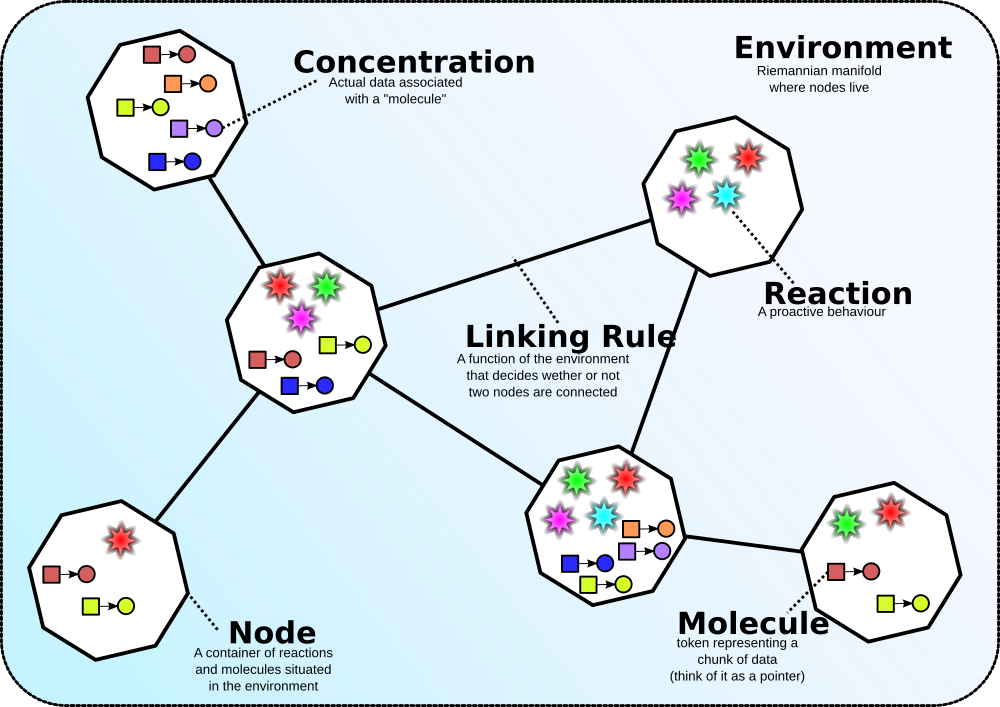
\includegraphics[width=.85\textwidth]{res/fig/alchemist_model.png}
          \caption[%
            Rappresentazione grafica delle diverse entità di Alchemist.
          ]{%
            Rappresentazione grafica delle diverse entità di Alchemist.\\
            Figura ripresa dal sito ufficiale\protect\footnotemark.
          }%
          \label{fig:alchemist:model}
        \end{figure}
        \footnotetext{\url{http://alchemistsimulator.github.io}}

      \item[Nodo]\label{itm:node}
        Il \emph{nodo} è un contenitore di \emph{molecole} e \emph{reazioni} che risiede all'interno di un \emph{ambiente} e che astrae una singola entità.

      \item[Ambiente]\label{itm:env}
        L'\emph{ambiente} è l'astrazione che rappresenta lo spazio nella simulazione ed è l'entità che contiene i \emph{nodi}.

        Esso è in grado di fornire informazioni in merito alla posizione dei \emph{nodi} nello spazio, alla distanza tra loro e al loro vicinato;
        opzionalmente, l'\emph{ambiente} può offrire il supporto allo spostamento dei \emph{nodi}.

      \item[Regola di collegamento]\label{itm:linkr}
        La \emph{regola di collegamento} è una funzione dello stato dell'\emph{ambiente} che associa ad ogni \emph{nodo} un \emph{vicinato}.

      \item[Vicinato]\label{itm:neigh}
        Un \emph{vicinato} è un'entità costituita da un \emph{nodo} detto ``centro'' e da un insieme di altri \emph{nodi} (i ``vicini'').

        L'astrazione dovrebbe avere un'accezione il più possibile generale e flessibile, in modo da poter modellare qualsiasi tipo di legame di vicinato, non solo spaziale.

        \begin{figure}[htbp]
          \centering
          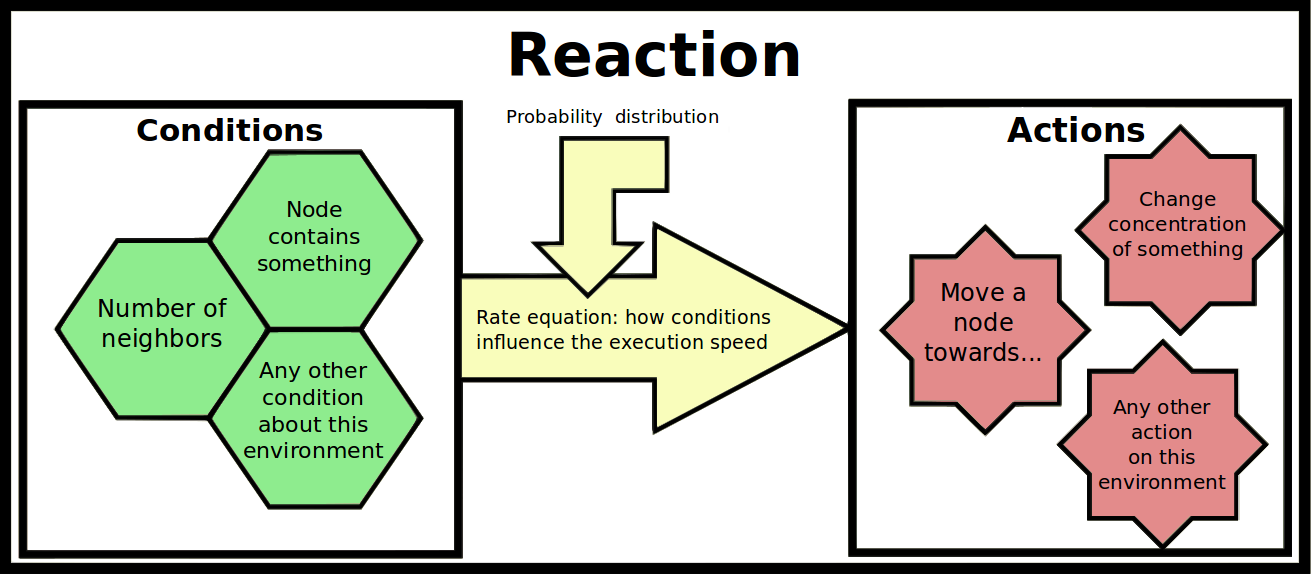
\includegraphics[width=.85\textwidth]{res/fig/alchemist_reaction.png}
          \caption{Rappresentazione grafica della \emph{Reazione}.}%
          \label{fig:alchemist:reaction}
        \end{figure}

      \item[Reazione]\label{itm:react}
        Il concetto di \emph{reazione} è da considerarsi molto più elaborato di quello utilizzato in chimica:
        in questo caso, si può considerare come un insieme di \emph{condizioni} sullo stato del sistema, che qualora dovessero risultare vere innescherebbero l'esecuzione di un insieme di \emph{azioni}.

        Una \emph{reazione} (di cui si ha una rappresentazione grafica in~\Cref{fig:alchemist:reaction}) è dunque un qualsiasi evento che può cambiare lo stato dell'\emph{ambiente} e si compone di un insieme di \emph{condizioni}, una o più \emph{azioni} e una distribuzione temporale.

        La frequenza di accadimento può dipendere da:
        \begin{itemize}
            \item Un tasso statico;
            \item Il valore di ciascuna \emph{condizione};
            \item Una equazione che combina il tasso statico e il valore delle \emph{condizioni}, restituendo un ``tasso istantaneo'';
            \item Una distribuzione temporale.
        \end{itemize}

        Ogni \emph{nodo} è costituito da un insieme (anche vuoto) di \emph{reazioni}.

      \item[Condizione]\label{itm:cond}
        Una \emph{condizione} è una funzione che associa un valore numerico e un valore booleano allo stato corrente di un \emph{ambiente}.

      \item[Azione]\label{itm:act}
        Un'\emph{azione} è una procedura che provoca una modifica allo stato dell'\emph{ambiente}.

    \end{description}

    Per quanto la terminologia sia ripresa dalla chimica, il meta-modello del simulatore è estendibile, adottando interpretazioni più o meno lasche dei termini ``molecola'' e ``concentrazione''.
    In particolare, in Alchemist esiste il concetto di \emph{incarnazione}, che definisce l'istanza concreta del meta-modello, delineando le modalità con le quali le astrazioni vengono implementate.

  \subsubsection{Incarnazione Protelis}

    Alchemist fornisce l'implementazione di diverse incarnazioni;
    per lo scopo di questa tesi, ci si propone di utilizzare l'incarnazione Protelis.
    In essa, la molecola identifica il nome di un sensore, mentre la sua concentrazione è il valore misurato.

    Attraverso la configurazione di Alchemist, è possibile definire il posizionamento dei nodi e le modalità di collegamento, nonché la presenza di specifiche molecole.
    In questo modo, è possibile definire una molecola che conterrà il codice Protelis che ciascun nodo deve eseguire;
    il sistema può così caricare dinamicamente il codice ottenendo la relativa concentrazione.
    Un esempio di configurazione è riportato in~\Cref{app:yaml}.


  \section{Interazioni}\label{sec:arch:interaction}

    \unsure[inline]{
      Ho deciso di descrivere le interazioni in una sezione dedicata, anziché separarle nelle sezioni del client e del server.

      È accettabile? O sarebbe meglio spezzare?
    }

    Una volta analizzato il comportamento delle due entità in gioco, è necessario delineare anche la loro interazione remota.

    \subsection{Scelta del modello di comunicazione e del protocollo}

      % Innanzitutto, è stato necessario chiarire quale tipo di comunicazione è necessario instaurare.
      Come detto nella \Cref{subsec:reactor}, per la progettazione del server di backend si è scelto di utilizzare un modello a event-loop multipli comunicanti tramite EventBus;
      inoltre, anche il pattern di gestione dello stato scelto per il funzionamento del client (\Cref{subsec:state-manage}) è event-driven.
      È risultato dunque naturale strutturare anche la comunicazione tra client e server utilizzando un modello a eventi.

      In particolare, l'EventBus di Vert.x supporta l'utilizzo di \emph{bridge} per la comunicazione remota attraverso numerosi protocolli.
      Tra questi, quello identificato come più adatto è \emph{SockJS}\@.

      SockJS è un protocollo pensato per realizzare una comunicazione \emph{WebSocket-like} sul maggior numero di piattaforme possibili.
      Esso gestisce in modo autonomo la verifica del supporto del protocollo WebSocket~\cite{Melnikov2011} da parte del client e del server, migrando su \emph{polling} tramite HTTP standard in caso assenza.
      Tramite un protocollo di questo tipo, è possibile realizzare un canale di comunicazione bidirezionale veloce, adatto per il trasferimento di un elevato numero di eventi come nel caso di questo progetto di tesi.

      Dunque, il \texttt{BridgeVerticle} esporrà tramite API (al percorso ``\texttt{/eventbus}'' relativamente all'\emph{host} principale) l'accesso all'EventBus per i messaggi previsti.
      L'applicazione web si dovrà connettere attraverso un client generando azioni sullo store interno.

    \subsection{Comportamento}

      Una volta chiarite le modalità di trasferimento delle informazioni, viene progettato il comportamento che permette al sistema di essere reattivo.
      In~\Cref{fig:event:vertx} viene rappresentata la sequenza di operazioni svolte dal server sulla base degli eventi inoltrati sull'EventBus di Vert.x;
      in~\Cref{fig:event:redux}, invece, il diagramma UML riassume la sequenza di azioni che permutano lo stato di Redux con il procedere dell'esecuzione.
      Di seguito, invece, sono riassunti i passaggi nel loro complesso.

      \begin{itemize}
        \item
          il primo passo è instaurare la connessione.
          La pressione di un bottone genera un'azione sullo store che abilita la connessione SockJS verso il backend.
          L'utente viene notificato del risultato dell'operazione attraverso la generazione, da parte del sistema, di azioni con le relative permutazioni dello stato.
          % In questo modo, l'interfaccia permette all'utente di trovare un backend valido e di collegarcisi attraverso socket.
        \item
          una volta che il codice Protelis è pronto per essere lanciato, l'utente utilizzerà il bottone dedicato per eseguirlo.
          Questo causa la creazione di un'azione di richiesta di upload del codice;
          esso è già presente nello store, dal quale viene prelevato e inoltrato tramite socket al server.
        \item
          il verticle riceve l'evento tramite EventBus;
          procede dunque costruendo un simulatore, al quale viene assegnato un identificativo univoco e un componente osservatore.
          Dopodiché, tramite EventBus viene inviato l'identificativo.
        \item
          il client riceve questo ID tramite socket e un'azione di Redux viene generata.
          La vista viene aggiornata di conseguenza, informando l'utente dell'avvenuta configurazione e dell'imminente avvio dell'esecuzione.
        \item
          quando il motore di simulazione esegue uno step, il componente osservatore viene notificato.
          Viene dunque generato un evento sul bus degli eventi diretto verso l'esterno, su un indirizzo legato all'identificativo iniziale e alla tipologia di variazione avvenuta nella simulazione (step iniziale, \emph{round} d'esecuzione, terminazione).
        \item
          quando l'esecuzione viene terminata sul simulatore, il client viene notificato dell'evento nello stesso modo con cui ha ricevuto i vari aggiornamenti.
          Sul server, l'ID verrà classificato come terminato e il simulatore potrà essere riutilizzato o distrutto a seconda delle necessità.
      \end{itemize}

      \begin{figure}[htbp]
        \centering
        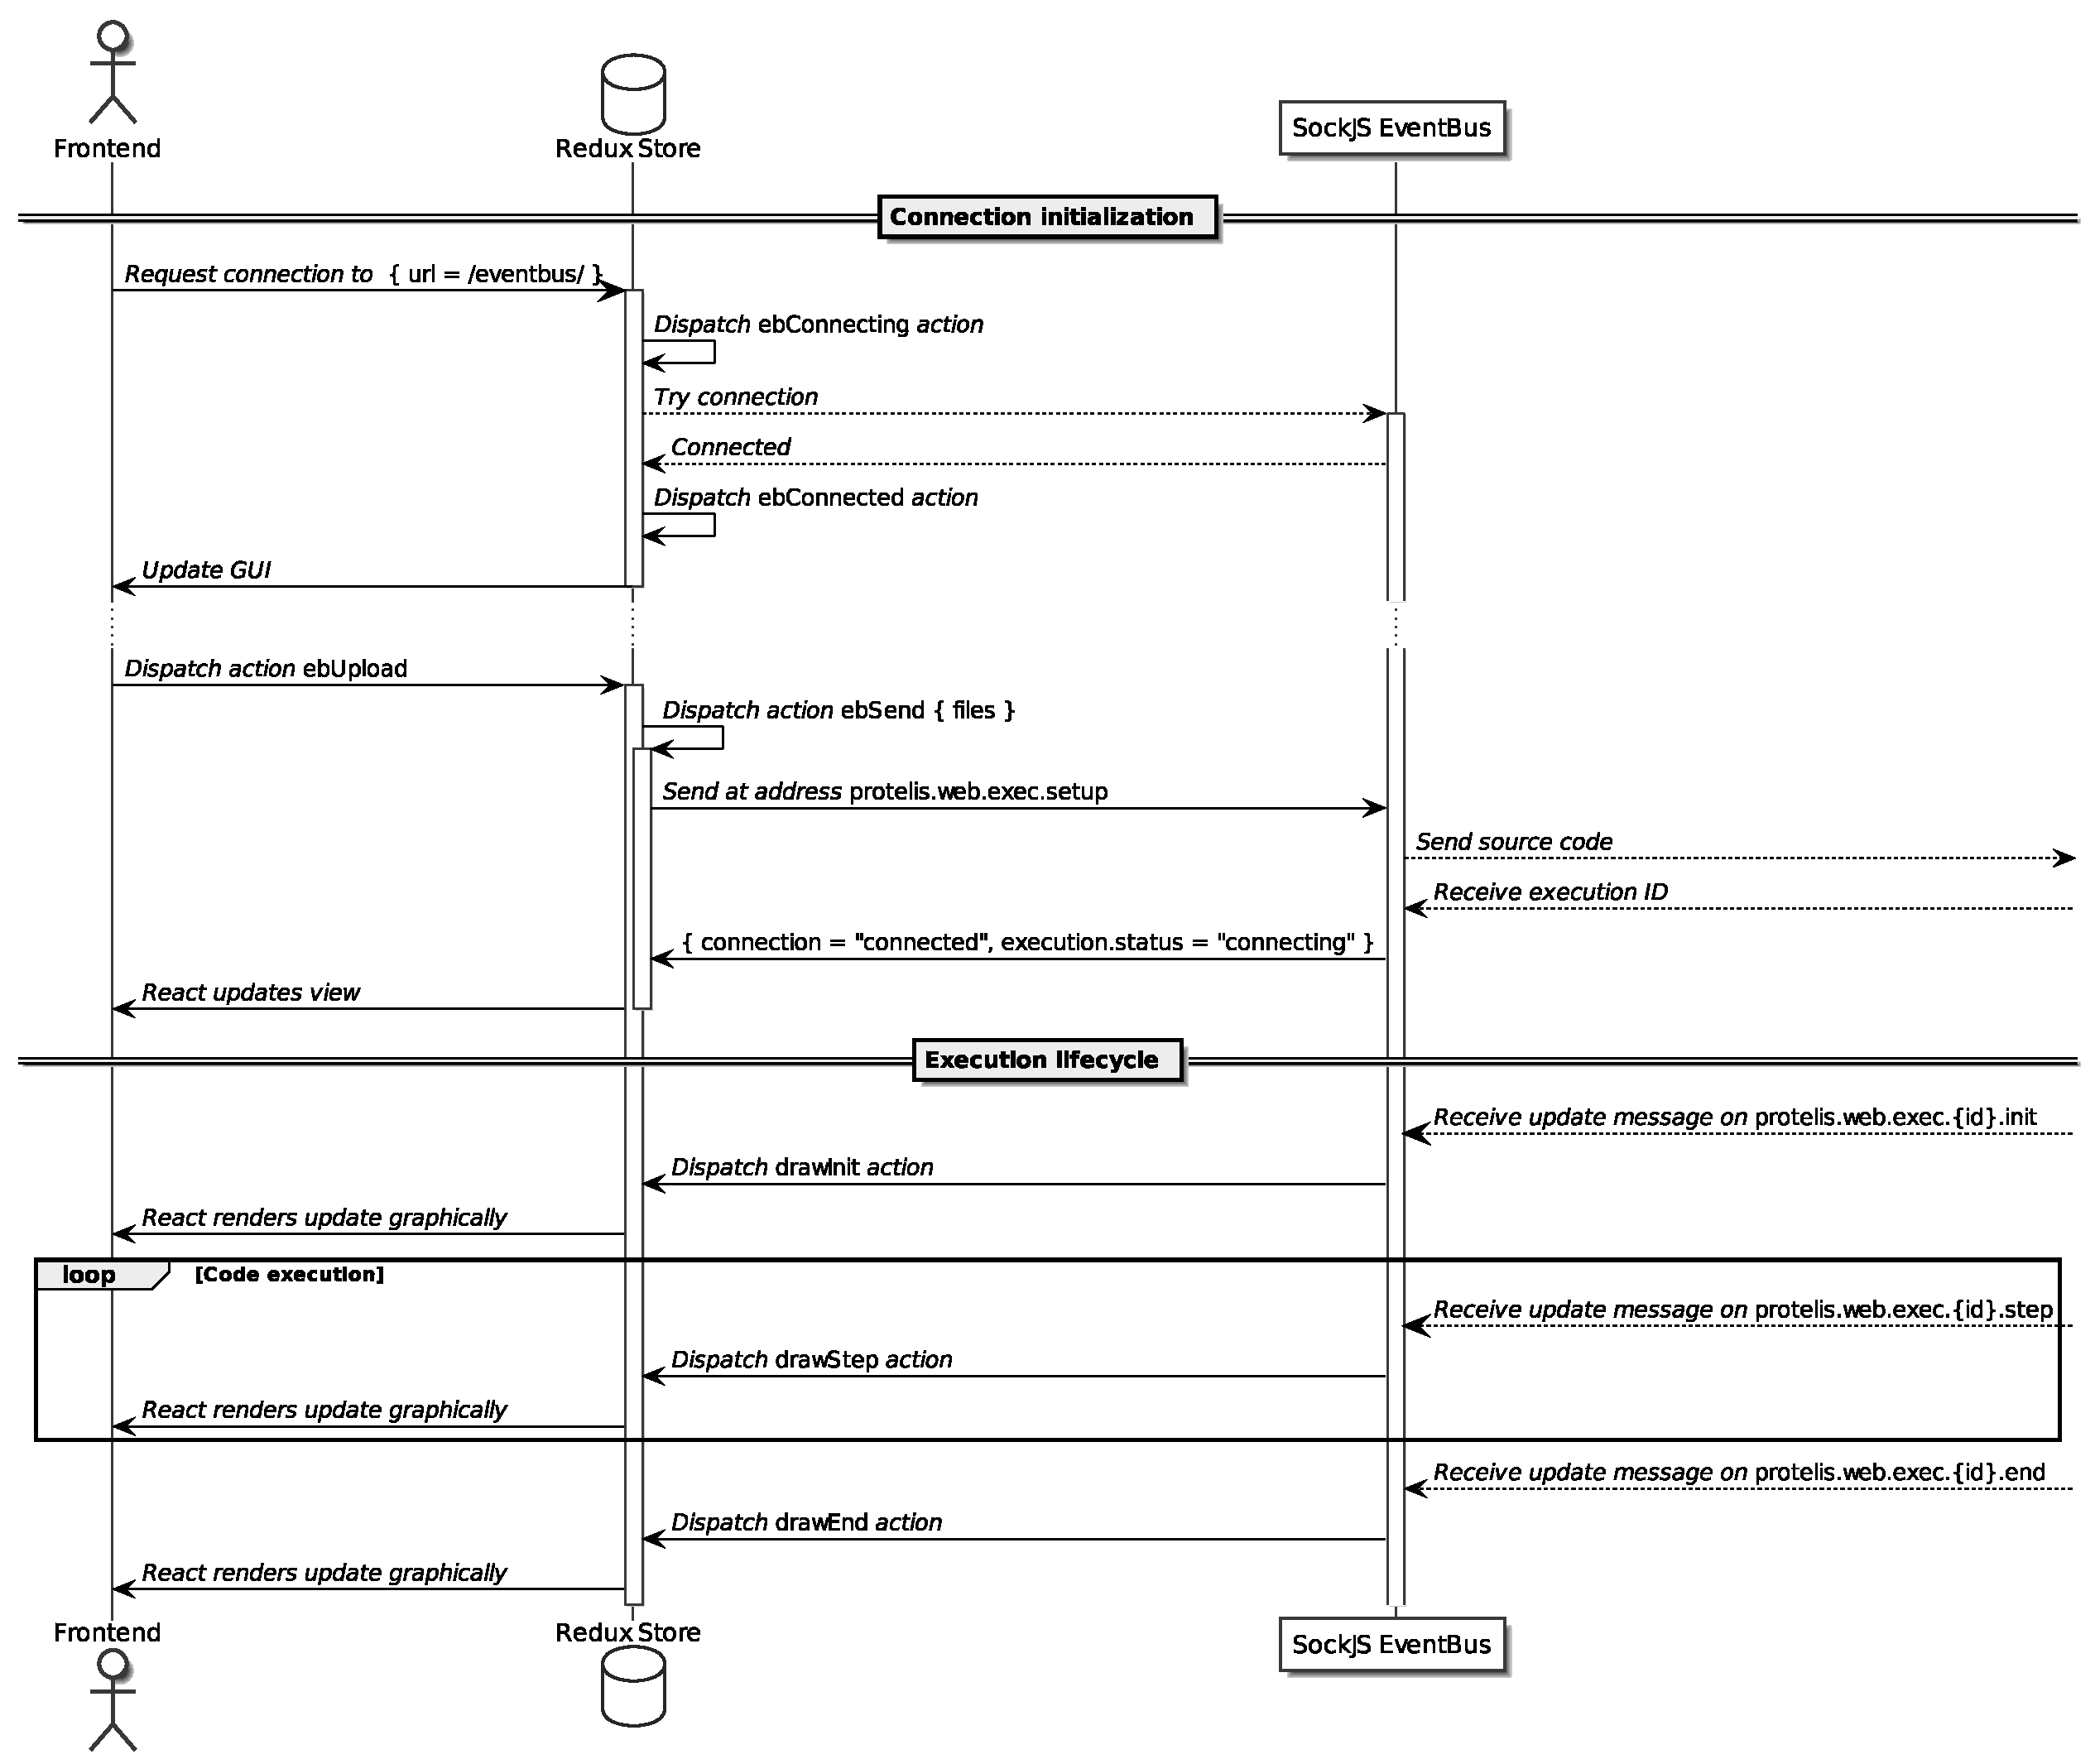
\includegraphics[width=.9\textwidth]{res/uml/redux-eventbus.eps}%
        \caption{Diagramma UML di sequenza rappresentante il flusso delle azioni sullo store di Redux.}%
        \label{fig:event:redux}
      \end{figure}

      \begin{figure}[htbp]
        \centering
        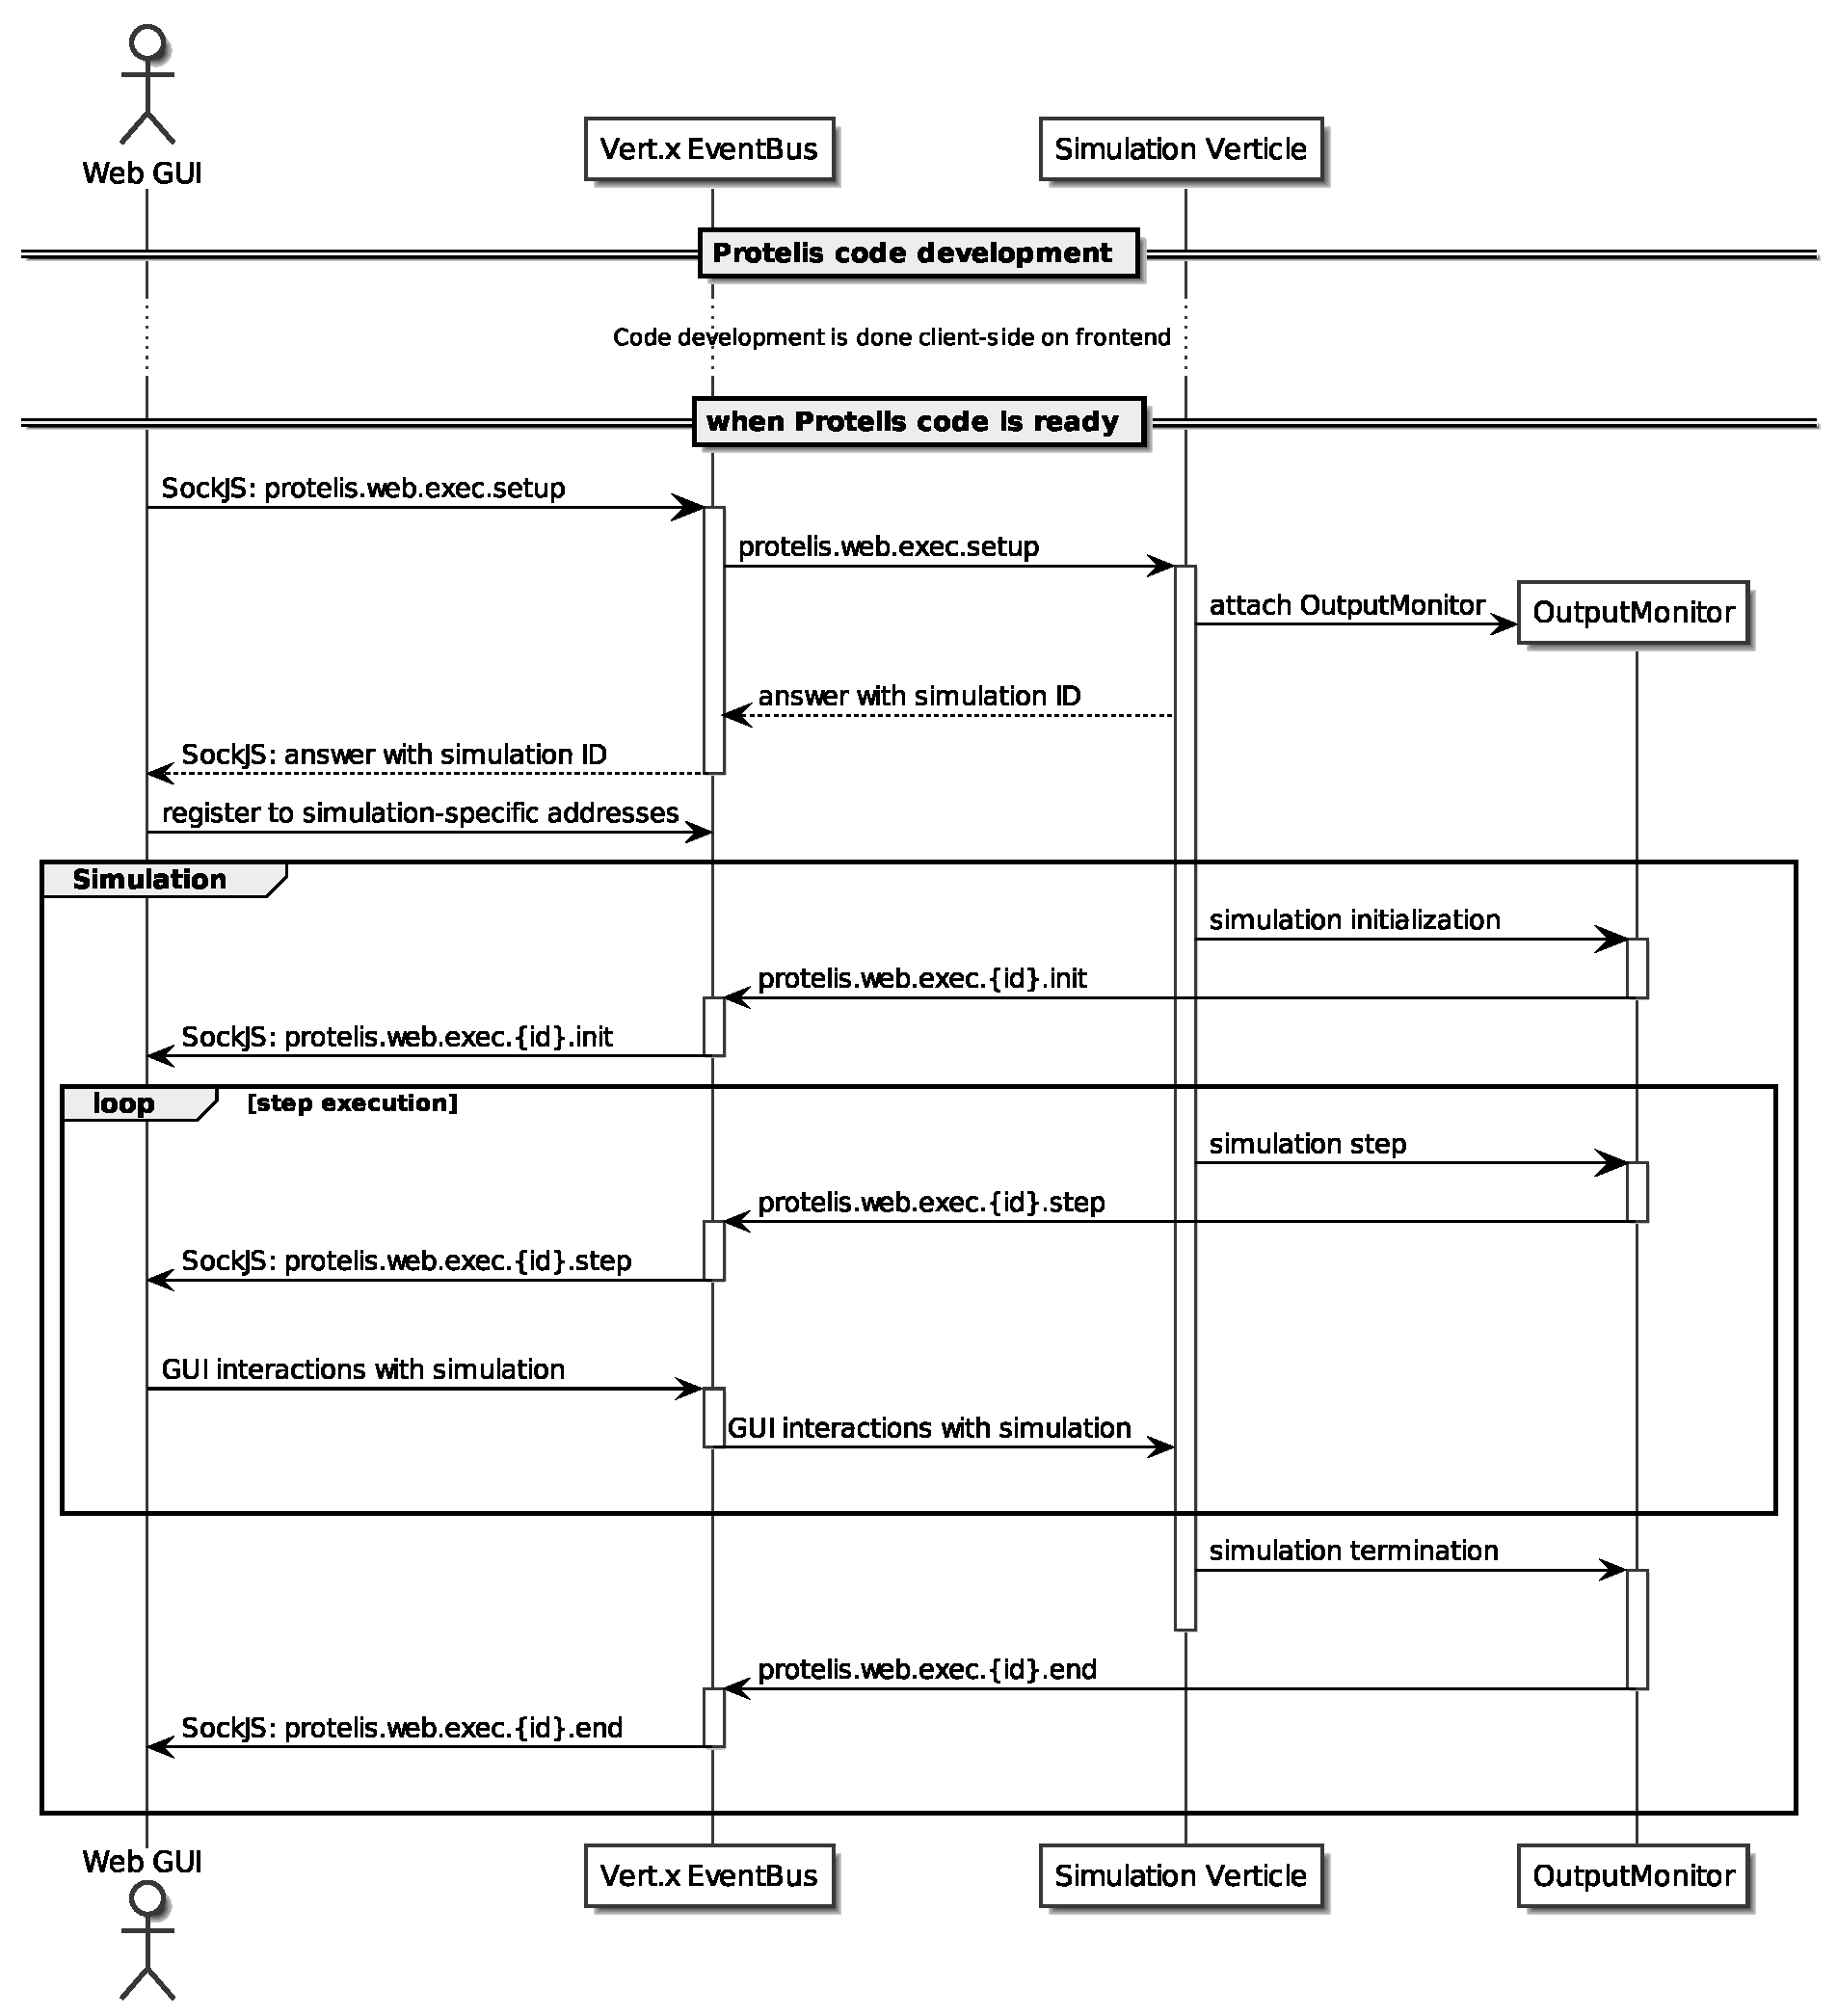
\includegraphics[width=.9\textwidth]{res/uml/data-flow.eps}%
        \caption{Diagramma UML di sequenza che rappresenta la gestione degli eventi sul bus di Vert.x.}%
        \label{fig:event:vertx}
      \end{figure}
